\chapter{Easy Hyperparameter Search Using Optunity}\label{ch:optunity}

\hyphenation{Optunity}
\newcommand{\optunity}{{\sc Optunity}\xspace}

\chapterfrontpagesubmitted{
Claesen, M., Simm, J., Popovic, D., Moreau, Y., \& De Moor, B. (2015). 
\textbf{Easy hyperparameter search using Optunity},
\emph{Journal of Machine Learning Research}.
}{
Marc Claesen has developed, maintained, tested and documented the software in Python, MATLAB and Octave and took the lead in writing the initial draft, the revision and rebuttal of the paper.
}{
    \optunity is a free software package dedicated to hyperparameter optimization. It contains various types of solvers, ranging from undirected methods to direct search, particle swarm and evolutionary optimization. The design focuses on ease of use, flexibility, code clarity and interoperability with existing software in popular machine learning environments. \optunity is written in Python and contains interfaces to R, Julia, Octave and MATLAB.  \optunity uses a BSD license and is available at \texttt{\url{http://www.optunity.net}}.
}

\section{Introduction}
Many machine learning tasks involve training a model $\mathcal{M}$ which minimizes some loss function $\mathcal{L}(\mathcal{M}\ |\ \test)$ on given test data $\test$. A model is obtained via a learning algorithm $\mathcal{A}$ which uses a training set $\train$ and solves some optimization problem. The learning algorithm $\mathcal{A}$ may itself be parameterized by a set of hyperparameters $\lambda$, e.g. $\mathcal{M} = \mathcal{A}(\train\ |\ \lambda)$.  Hyperparameter search -- also known as tuning -- aims to find a set of hyperparameters $\lambda^*$, such that the learning algorithm yields an optimal model $\mathcal{M}^*$ that minimizes $\mathcal{L}(\mathcal{M}\ |\ \test)$:
\begin{equation}
\lambda^* = \argmin_{\lambda} \mathcal{L}\big(\mathcal{A}(\train\ |\ \lambda)\ |\ \test\big) = \argmin_{\lambda} \obj(\lambda\ |\ \mathcal{A},\ \train, \test,\ \mathcal{L}). \label{equation}
\end{equation}
In tuning, $\obj$ is the objective function and the hyperparameters $\lambda$ are optimization variables. The learning algorithm $\mathcal{A}$, loss function $\mathcal{L}$ and data sets $\train$ and $\test$ are known. %Depending on the learning task, $\train$ and $\test$ may be labeled and/or equal to each other. The objective function often has a constrained domain (for example regularization terms must be positive) and is assumed to be expensive to evaluate, black-box and non-smooth.

Tuning hyperparameters is a recurrent task in machine learning which may significantly affect overall performance. Commonly tuned hyperparameters are related to kernels, regularization, learning rates and network architecture. Some specific challenges associated to hyperparameter optimization are discussed by Claesen and De Moor \citep{claesen2015hyperparameter}. General machine learning packages provide only basic tuning methods like grid search \citep{pedregosa2011scikit}. In practice, the most common tuning approaches are grid search and manual tuning, though both are known to fail when the number of hyperparameters grows and manual search is additionally hard to reproduce \citep{bergstra2012random}.

The current adoption of dedicated hyperparameter optimizers is limited: we surveyed NIPS 2014 and found that only 2 out of 86 works used suitable approaches while 84 papers reported the use of grid search, random search or manual tuning (cfr. Appendix~\ref{survey}).


\section{Optunity}
\optunity offers various optimizers and utility functions to enable efficient hyperparameter optimization using only a few of lines of code and minimal expertise. Our software is complementary to libraries that provide learning algorithms, such as \textsc{scikit-learn} \citep{pedregosa2011scikit}. The package uses a BSD license and is simple to deploy in any environment. \optunity supports Python, R, Octave and MATLAB on Linux, OSX and Windows.

\subsection{Functional Overview}
\optunity provides both simple routines for lay users and expert routines that enable fine-grained control of various aspects of the solving process. Basic tuning requires only an objective function, a maximum number of evaluations and box constraints on the hyperparameters to be optimized. Conditional search spaces in which the existence of some hyperparameters is contingent upon some discrete choice are also supported.

The objective function must be defined by the user. It takes a hyperparameter tuple $\lambda$ and typically involves three steps: (i) training a model $\mathcal{M}$ with $\lambda$, (ii) use $\mathcal{M}$ to predict a test set and (iii) compute some score or loss based on the predictions. %In unsupervised tasks, the separation between (i) and (ii) need not exist, for example in clustering a data set.

Tuning involves a series of function evaluations until convergence or until a predefined maximum number of evaluations is reached. \optunity is capable of vectorizing evaluations in the working environment to speed up the process at the end user's volition.

\optunity also provides $k$-fold cross-validation to estimate the generalization performance of supervised modeling approaches. The implementation can account for strata and clusters.\footnote{Instances in a stratum should be spread across folds. Clustered instances must remain in a single fold.} Finally, a variety of common quality metrics is available. 
The snippet below shows how to tune an SVM classifier with RBF kernel using {\sc scikit-learn} and \optunity:\footnote{We assume the correct imports are made and \texttt{data} and \texttt{labels} contain appropriate content.}


\begin{lstlisting}[style=Py, frame=none, xleftmargin=1.5ex, escapeinside={(*@}{@*)}]
!@optunity.cross_validated!(x=(*@\textcolor{red}{data}@*), y=(*@\textcolor{red}{labels}@*), num_folds=10, num_iter=2)
def (*@\textcolor{blue}{score}@*)(x_train, y_train, x_test, y_test, (*@\textcolor{blue}{C}@*), (*@\textcolor{blue}{gamma}@*)):
    model = sklearn.svm.SVC(C=10**(*@\textcolor{blue}{C}@*), gamma=10**(*@\textcolor{blue}{gamma}@*)).fit(x_train, y_train)
    decision_values = model.decision_function(x_test)
    return !optunity.metrics.roc_auc!(y_test, decision_values)

!hps!, _, _ = !optunity.maximize!((*@\textcolor{blue}{score}@*), num_evals=100, (*@\textcolor{blue}{C=[-5, 2]}@*), (*@\textcolor{blue}{gamma=[-5, 0]}@*)) (*@\label{optunity-maximize}@*)
svm = sklearn.svm.SVC(C=10**!hps['C']!, gamma=10**!hps['gamma']!) (*@\label{train-tuned-svm1}@*)
svm.fit((*@\textcolor{red}{data}@*), (*@\textcolor{red}{labels}@*)) (*@\label{train-tuned-svm2}@*)
\end{lstlisting}

The objective function as per Equation~\eqref{equation} is defined on lines 1 to 5, where $\lambda = (C, \gamma)$, $\mathcal{A}$ is the SVM training algorithm and $\mathcal{L}$ is area under the ROC curve. We use $2\times$ iterated 10-fold cross-validation to estimate area under the ROC curve. Up to $100$ hyperparameter tuples are tested in an exponential search space, bounded by $10^{-5} < C < 10^2$ and $10^{-5} < \gamma < 10^0$ on line \ref{optunity-maximize}. Finally, an SVM with optimized hyperparameters is trained on lines \ref{train-tuned-svm1} and \ref{train-tuned-svm2}.


\subsection{Available Solvers}
\optunity provides a wide variety of solvers, ranging from basic, undirected methods like grid search, sobol sequences and random search \citep{bergstra2012random} to evolutionary methods such as particle swarm optimization \citep{kennedy2010particle}, the covariance matrix adaptation evolutionary strategy (CMA-ES) \citep{hansen2001completely}, tree-structured Parzen estimator \citep{bergstra2011algorithms} and the Nelder-Mead simplex. The default solver is particle swarm optimization, which performs well for a large variety of tuning tasks involving various learning algorithms. Additional solvers will be incorporated in the future.
 
\subsection{Software Design and Implementation}

The design philosophy of \optunity prioritizes code clarity over performance. This is justified by the fact that objective function evaluations constitute the performance bottleneck. 

In contrast to typical Python packages, we avoid dependencies to facilitate users working in non-Python environments (sometimes at the cost of performance). To prevent issues for users that are unfamiliar with Python, care is taken to ensure all code in \optunity works out of the box on any Python version above 2.7, without requiring tools like \texttt{2to3} to make explicit conversions. \optunity has optional dependencies on {\sc DEAP} \citep{fortin2012deap} and {\sc Hyperopt} \citep{bergstra2013hyperopt} for the CMA-ES and TPE solvers, respectively. 

A key aspect of \optunity's design is interoperability with external environments. This requires bidirectional communication between \optunity's Python back-end ($\mathcal{O}$) and the external environment ($\mathcal{E}$) and roughly involves three steps: (i) $\mathcal{E}\rightarrow\mathcal{O}$ solver configuration, (ii) $\mathcal{O}\leftrightarrow\mathcal{E}$ objective function evaluations and (iii) $\mathcal{O}\rightarrow\mathcal{E}$ solution and solver summary. To this end, \optunity can do straightforward communication with any environment via sockets using JSON messages as shown in Figure~\ref{fig:workflow}. Only some information must be communicated, big objects like data sets are never exchanged. To port \optunity to a new environment, a thin wrapper must be implemented to handle communication.

\begin{figure}[!h]
  \centering 
      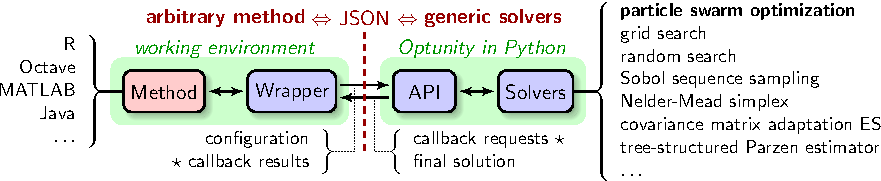
\includegraphics[width=\textwidth]{software.pdf} 
  \caption{Integrating \optunity in non-Python environments.}\label{fig:workflow}
\end{figure}

\subsection{Development and Documentation}
Collaborative development is organized via GitHub.\footnote{We maintain the following subdomains for convenience: \texttt{http://}$\{$\href{http://builds.optunity.net}{builds}, \href{http://docs.optunity.net}{docs}, \href{http://git.optunity.net}{git}, \href{http://issues.optunity.net}{issues}$\}$\texttt{.optunity.net}.} The project's master branch is kept stable and is subjected to continuous integration tests using Travis CI. 
We recommend prospective users to clone the master branch for the most up-to-date stable version of the software. Bug reports and feature requests can be filed via issues on GitHub. Future development efforts will focus on wrappers for Java and C/C++. We additionally plan to incorporate Bayesian optimizers which have no reference implementation in other packages. %Bayesian optimization strategies that are unavailable elsewhere \citep{jones1998efficient}. 

Code is documented using Sphinx and contains many doctests that can serve as both unit tests and examples of the associated functions. 
Our website contains developer and user documentation and a wide range of examples to illustrate all aspects of the software. 
The examples involve various packages and environments, including \textsc{scikit-learn} \citep{pedregosa2011scikit}, \textsc{OpenCV} \citep{opencv_library} and \textsc{Spark}'s \textsc{MLlib} \citep{zaharia2010spark}.
%Finally, some practical applications are available, including object recognition using OpenCV \citep{opencv_library} and deep learning with Theano \citep{bergstra2011theano}. % and semisupervised learning \citep{claesen2014robust}.

%\section{Conclusions}
%Optunity contains a variety of optimization methods that can be used for hyperparameter search. Using proper search methods becomes particularly important for machine learning methods with many hyperparameters, such as convolutional networks, deep belief networks and ensembles of SVM models.

\section{Related Work}

A number of software solutions exist for hyperparameter search. \textsc{Hyperopt} offers random search and sequential model-based optimization \citep{bergstra2013hyperopt}. Some packages dedicated to Bayesian approaches include \textsc{Spearmint} \citep{snoek2012practical}, \textsc{DiceKriging} \citep{roustant2012dicekriging}, \textsc{SMAC} \citep{hutter2011sequential} and \textsc{BayesOpt} \citep{martinez2014bayesopt}. Finally, \textsc{ParamILS} provides iterated local search \citep{hutter2009paramils}. 

%Existing packages tend to be one-trick ponies, providing a specific class of optimization methods and offering limited support to users in different machine learning environments. 
\optunity distinguishes itself from other packages by exposing a variety of fundamentally different solvers through a lightweight API. \optunity's client-server model facilitates integration in any language and environment and can even be used to run solvers remotely.

\section{Solver Benchmark}
We compared Optunity against BayesOpt \citep{martinez2014bayesopt}, Hyperopt \citep{bergstra2013hyperopt}, SMAC \citep{hutter2011sequential}, and random search \citep{bergstra2012random}. Implementations of the last three solvers were available in HPOlib \citep{eggensperger2013towards}. We optimized 5-fold cross-validated area under the ROC curve for an SVM classifier with an RBF kernel (with continuous hyperparameters $\log C$ and $\log \gamma$), given a fixed search space and a budget of 150 evaluations on 19 pristine real-world problems. All solvers were given identical objective functions. Figure~\ref{fig:benchmark} summarizes the results using critical difference (CD) diagrams as introduced by Dem{\v{s}}ar \citep{demvsar2006statistical}. More details are available in Appendix~\ref{optunity:benchmark}.%\footnote{The benchmark implementation is available at \url{https://github.com/claesenm/optunity-benchmark}.}

Optunity and BayesOpt statistically significantly outperformed random search at 75 and 150 evaluations, with BayesOpt winning twice. Optunity improved at 150 evaluations relative to the other optimizers, indicating it is better at local search. Overall, we conclude that all 4 directed optimizers are competitive and convincingly outperform random search.


%PSO has also been shown to be competitive to TPE in tuning RBMs by \citet{papa2015model}.

\begin{figure}[!h]
  \centering 
      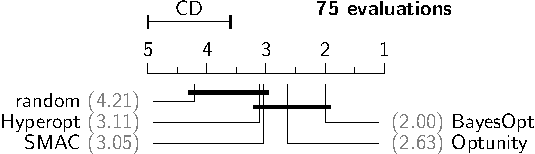
\includegraphics[width=0.6\textwidth]{cd_75.pdf} \\
      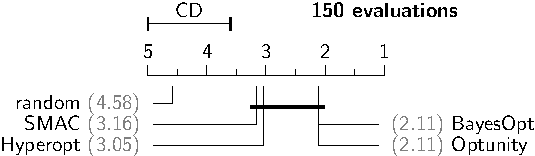
\includegraphics[width=0.6\textwidth]{cd_150.pdf}
\caption{Critical difference diagrams for 75 and 150 evaluations to tune an SVM with RBF kernel, depicting average rank per optimizer (lower is better). Optimizers without statistically significant performance differences at $\alpha=5\%$ are linked.}\label{fig:benchmark}
\end{figure}

\begin{subappendices}

\section{Survey of hyperparameter optimization in NIPS 2014} \label{survey}
To objectively assess the current adoption of dedicated hyperparameter optimization techniques, we have surveyed all papers of the NIPS 2014 conference\footnote{The NIPS 2014 conference homepage is available at \url{https://nips.cc/Conferences/2014/}.} (411 in total).\footnote{The full survey with each paper's tags is available at \url{https://github.com/jaak-s/nips2014-survey}.} The main question was how many papers reported the use of techniques other than grid search, random search and manual tuning. We counted all papers mentioning cross-validation or hyperparameter optimization (86 papers) and then categorized these papers based on which hyperparameter optimization method was used. Table~\ref{table:survey} summarizes the survey's outcome.\footnote{To automate the survey and make it reproducible, we scanned all papers for names of well-known hyperparameter optimization packages and techniques along with names of the authors of the corresponding publications. Using this approach, we automatically accounted for random search \citep{bergstra2012random}, Spearmint \citep{snoek2012practical}, Hyperopt \citep{bergstra2013hyperopt}, BayesOpt \citep{martinez2014bayesopt}, ParamILS \citep{hutter2009paramils}, SMAC \citep{hutter2011sequential} and the Tree of Parzen Estimators (TPE) optimizer \citep{bergstra2011algorithms}.}

\begin{table}[!h]
\centering
\begin{tabular}{ll}
\toprule
\textbf{optimization method} & \textbf{number of uses} \\
\midrule
grid search & 82 \\
random search & 2 \\
Spearmint \citep{snoek2012practical} & 1 \\
predictive entropy search \citep{hernandez2014predictive} & 1  \\
\midrule
\textbf{total} & \textbf{86} \\
\bottomrule
\end{tabular}
\caption{The use of hyperparameter optimization methods as reported in NIPS 2014 papers. Methods and packages with 0 recorded uses are omitted from this table.} \label{table:survey}
\end{table}

Table~\ref{table:survey} indicates that the adoption of dedicated hyperparameter optimizers remains limited in contemporary machine learning. Grid search remains the head honcho for hyperparameter optimization (used in 82 out of 86 works, or $95\%$), despite significant evidence that better optimization methods exist. Although automated hyperparameter optimization is a hot topic in contemporary machine learning research, the resulting methods appear to not yet be a part of practitioners' toolkits and workflows (used in 2 out of 86 works, or $2\%$). 

We believe several barriers exist towards the adoption of dedicated hyperparameter optimization methods. First, users must know of their existence and relative benefit compared to conventional methods (we believe this to be the case). Second, these methods must be available in all common machine learning environments. Third, it must be easy for potential users to start using these optimizers and get immediate results, which requires that installation is straightforward and the APIs are intuitive, flexible and well-documented.

Finally, it is worth noting that NIPS is one of the hotspots of automated hyperparameter optimization research, both in terms of publications and related workshops. Hence it is reasonable to assume that the adoption of dedicated hyperparameter optimization methods is elevated within the NIPS community compared to the entire machine learning field and more applied fields such as computer vision and bioinformatics.


%%%%%%%%%%%%%%%%%%%%%%%%%%%%%%%%%%%%%%%%
%
%	BENCHMARK
%
%%%%%%%%%%%%%%%%%%%%%%%%%%%%%%%%%%%%%%%%


\section{Performance benchmark} \label{optunity:benchmark}
We created a benchmark to assess the performance of Optunity's default optimizer (particle swarm optimization) against the defaults of SMAC \citep{hutter2011sequential}, Hyperopt \citep{bergstra2013hyperopt} and BayesOpt \citep{martinez2014bayesopt} for real hyperparameter search tasks.\footnote{The benchmark is based on HPOlib (which provided Hyperopt, SMAC and random search). All code and full results are available at \url{https://github.com/claesenm/optunity-benchmark} and should work on any linux platform, provided all dependencies are met.}

\subsection{Setup}
Our benchmark entails optimizing the 2 continuous hyperparameters of an SVM classifier with RBF kernel on an exponential grid ($10^{-8} < C < 10$ and $10^{-8} < \gamma < 10$). We used 5-fold cross-validation to estimate area under the ROC curve to build the objective function. All optimizers used the exact same objective function and a uniform prior to optimize $\log_{10}(C)$ and $\log_{10}(\gamma)$ within the specified bounds (the exponentiation was done within the objective function). Each optimizer was given a budget of 150 function evaluations and we probed their intermediate results at 75 evaluations and the final results at 150 evaluations.

We simulated 19 real-world problems based on the \texttt{mnist digits}, \texttt{covtype}, \texttt{diabetes} and \texttt{ionosphere} data sets. Multiclass data sets were used several times in a one-vs-all setting, i.e., \texttt{mnist digits} and \texttt{covtype} were used to create 10 and 7 optimization problems, respectively. \texttt{mnist digits} and \texttt{covtype} were used as provided in scikit-learn \citep{pedregosa2011scikit}, while we used the scaled versions of the \texttt{diabetes} and \texttt{ionosphere} data sets as available on the website of LIBSVM.\footnote{Available at \url{https://www.csie.ntu.edu.tw/~cjlin/libsvmtools/datasets/} and in the GitHub repo.} 

For some data sets we added random noise on the data matrix to make the learning problems more challenging and enable differentiating between various hyperparameter optimizers. Each task was simulated 5 times to improve consistency. Results of each optimization task at 75 and 150 evaluations are shown in Tables~\ref{table:benchmark-results-75} and \ref{table:benchmark-results-150}, respectively, which show average performance and rank of each solver per data set along with an overall summary.

\subsection{Results \& Discussion}
The results of the benchmark are summarized in Figure~\ref{fig:benchmark} and shown in full for 75 and 150 evaluations in Tables~\ref{table:benchmark-results-75} and \ref{table:benchmark-results-150}, respectively. The tables show averages (across 5 runs per problem) of the optimum across all solvers, the third quantile of random search performance (to indicate problem difficulty) and the relative rank and regret per solver. Regret in this case means the difference between an optimizer's best and the overall best solution in a given experiment and can be considered to measure the cost of using a given optimizer for a given task, with the optimizer that found the best solution inducing 0 regret.

Overall, BayesOpt took the lead in this benchmark at both evaluation counts, followed by Optunity. Optunity and Hyperopt improve in terms of regret and relative rank in evaluations 76--150, with Optunity showing the biggest relative improvement. Since most optimizers have already reached fairly good solutions after 75 evaluations, local search performance is key in the final 75 evaluations. Since Optunity's regret and relative rank amongst optimizers show a noteworthy improvement at 150 evaluations compared to 75 evaluations, we conclude that its local search performance beats that of other optimizers.

\begin{landscape}
\begin{table}[!h]
\caption{Benchmark results for tuning an SVM classifier with RBF kernel, using an optimization budget of 75 evaluations (best result per data set in bold, worst in gray). Results depict averages across 5 runs of the optimum (i.e., the best found solution across all optimizers), the third quantile ($Q_3$) of random search results (which indicates the difficulty of the optimization problem: low $Q_3$ vis-\`a-vis the optimum indicates the region of strong performance is small within the overall search space) and the relative rank and regret per optimizer. Performance and regret are measured in terms of cross-validated area under the ROC curve and shown in percent. Relative ranks indicate non-parametric global performance within the pool of optimizers (lower is better, the best optimizer has rank 1).}
\label{table:benchmark-results-75}
\centering
\resizebox{1.4\textwidth}{!}{%
\begin{tabular}{lcccccccccccccccccc}
\toprule
 & & & & \multicolumn{2}{c}{Optunity} & & \multicolumn{2}{c}{Hyperopt} & & \multicolumn{2}{c}{SMAC} & & \multicolumn{2}{c}{BayesOpt} & & \multicolumn{2}{c}{random search} \\\cline{5-6} \cline{8-9} \cline{11-12} \cline{14-15} \cline{17-18}
data set & optimum & $Q_3$ & & rank & regret & & rank & regret & & rank & regret & & rank & regret & & rank & regret \\
\midrule
\texttt{digits-0} & 96.56 & 95.46 & & \textbf{1.80} & \textbf{0.041} & & 3.20 & 0.096 & & 3.40 & 0.145 & & \textbf{1.80} & 0.055 & & {\color{gray}4.80} & {\color{gray}0.340}\\
\texttt{digits-1} & 91.10 & 86.69 & & 2.40 & 0.256 & & 2.60 & 0.258 & & 3.80 & 0.562 & & \textbf{1.20} & \textbf{0.069} & & {\color{gray}5.00} & {\color{gray}1.064}\\
\texttt{digits-2} & 93.27 & 91.19 & & 2.60 & 0.166 & & 3.80 & 0.376 & & 2.60 & 0.390 & & \textbf{2.00} & \textbf{0.156} & & {\color{gray}4.00} & {\color{gray}0.734}\\
\texttt{digits-3} & 90.82 & 88.63 & & 2.20 & 0.316 & & 3.40 & 0.530 & & 3.40 & 0.528 & & \textbf{1.80} & \textbf{0.093} & & {\color{gray}4.20} & {\color{gray}0.651}\\
\texttt{digits-4} & 94.86 & 93.50 & & 3.60 & 0.406 & & 3.20 & 0.291 & & 2.20 & 0.222 & & \textbf{1.60} & \textbf{0.051} & & {\color{gray}4.40} & {\color{gray}0.480}\\
\texttt{digits-5} & 93.11 & 90.67 & & 2.60 & 0.328 & & 3.60 & 0.570 & & 2.40 & 0.399 & & \textbf{1.40} & \textbf{0.101} & & {\color{gray}5.00} & {\color{gray}1.038}\\
\texttt{digits-6} & 95.97 & 94.97 & & 3.40 & 0.325 & & 2.20 & 0.121 & & 3.20 & 0.300 & & \textbf{1.60} & \textbf{0.098} & & {\color{gray}4.60} & {\color{gray}0.516}\\
\texttt{digits-7} & 95.20 & 93.52 & & 3.00 & 0.162 & & 2.80 & 0.193 & & 2.20 & 0.130 & & \textbf{2.00} & \textbf{0.068} & & {\color{gray}5.00} & {\color{gray}0.774}\\
\texttt{digits-8} & 82.75 & 73.61 & & 3.00 & 0.365 & & 2.80 & 0.370 & & {\color{gray}3.80} & {\color{gray}0.754} & & \textbf{1.80} & \textbf{0.168} & & 3.60 & 0.373\\
\texttt{digits-9} & 87.92 & 84.61 & & 2.60 & 0.260 & & 2.60 & 0.506 & & 3.20 & 0.522 & & \textbf{1.60} & \textbf{0.164} & & {\color{gray}5.00} & {\color{gray}1.143}\\
\texttt{covtype-1} & 82.41 & 77.44 & & \textbf{2.00} & 0.508 & & 3.20 & 0.870 & & 3.00 & 0.868 & & 2.60 & \textbf{0.442} & & {\color{gray}4.20} & {\color{gray}1.491}\\
\texttt{covtype-2} & 81.97 & 73.97 & & 2.20 & 0.649 & & 2.80 & 0.919 & & 3.80 & 2.074 & & \textbf{1.60} & \textbf{0.262} & & {\color{gray}4.60} & {\color{gray}2.906}\\
\texttt{covtype-3} & 97.91 & 94.79 & & 3.20 & {\color{gray}0.263} & & 3.20 & 0.210 & & {\color{gray}3.60} & 0.185 & & \textbf{1.60} & \textbf{0.012} & & 3.40 & 0.182\\
\texttt{covtype-4} & 99.76 & 98.40 & & 3.20 & {\color{gray}0.130} & & 3.40 & 0.058 & & 3.20 & 0.090 & & \textbf{1.60} & \textbf{0.019} & & {\color{gray}3.60} & 0.067\\
\texttt{covtype-5} & 96.84 & 90.53 & & {\color{gray}4.00} & {\color{gray}0.797} & & 2.80 & 0.441 & & 3.00 & 0.586 & & \textbf{1.20} & \textbf{0.023} & & {\color{gray}4.00} & 0.744\\
\texttt{covtype-6} & 97.40 & 93.63 & & {\color{gray}4.60} & {\color{gray}0.595} & & 2.80 & 0.241 & & 2.40 & 0.339 & & \textbf{1.40} & \textbf{0.083} & & 3.80 & 0.498\\
\texttt{covtype-7} & 98.51 & 94.66 & & 2.80 & 0.183 & & 3.00 & 0.335 & & {\color{gray}4.80} & {\color{gray}0.854} & & \textbf{1.00} & \textbf{0.000} & & 3.40 & 0.440\\
\texttt{diabetes} & 84.28 & 81.87 & & 3.60 & 0.785 & & 2.00 & 0.293 & & 2.60 & 0.220 & & \textbf{1.80} & \textbf{0.163} & & {\color{gray}5.00} & {\color{gray}1.477}\\
\texttt{ionosphere} & 83.20 & 73.90 & & \textbf{2.00} & 0.650 & & 2.60 & 0.681 & & 3.40 & 1.409 & & 2.60 & \textbf{0.606} & & {\color{gray}4.40} & {\color{gray}1.682}\\
\midrule
average & N/A & N/A & & 2.88 & 0.378 & & 2.95 & 0.387 & & 3.16 & 0.557 & & \textbf{1.69} & \textbf{0.139} & & {\color{gray}4.32} & {\color{gray}0.874} \\
\bottomrule
\end{tabular}%
}
\end{table}

\begin{table}[!h]
\caption{Benchmark results for tuning an SVM classifier with RBF kernel, using an optimization budget of 150 evaluations (best result per data set in bold, worst in gray). Results depict averages across 5 runs of the optimum (i.e., the best found solution across all optimizers), the third quantile ($Q_3$) of random search results (which indicates the difficulty of the optimization problem: low $Q_3$ vis-\`a-vis the optimum indicates the region of strong performance is small within the overall search space) and the relative rank and regret per optimizer. Performance and regret are measured in terms of cross-validated area under the ROC curve and shown in percent. Relative ranks indicate non-parametric global performance within the pool of optimizers (lower is better, the best optimizer has rank 1).}
\label{table:benchmark-results-150}
\centering
\resizebox{1.4\textwidth}{!}{%
\begin{tabular}{lcccccccccccccccccc}
\toprule
 & & & & \multicolumn{2}{c}{Optunity} & & \multicolumn{2}{c}{Hyperopt} & & \multicolumn{2}{c}{SMAC} & & \multicolumn{2}{c}{BayesOpt} & & \multicolumn{2}{c}{random search} \\\cline{5-6} \cline{8-9} \cline{11-12} \cline{14-15} \cline{17-18}
data set & optimum & $Q_3$ & & rank & regret & & rank & regret & & rank & regret & & rank & regret & & rank & regret \\
\midrule
\texttt{digits-0} & 96.68 & 95.41 & & 2.40 & 0.065 & & 3.40 & 0.110 & & 2.40 & 0.157 & & \textbf{1.80} & \textbf{0.043} & & {\color{gray}5.00} & {\color{gray}0.391}\\
\texttt{digits-1} & 91.26 & 86.48 & & 3.20 & 0.371 & & \textbf{1.80} & 0.182 & & 3.20 & 0.477 & & 2.00 & \textbf{0.095} & & {\color{gray}4.80} & {\color{gray}0.726}\\
\texttt{digits-2} & 93.42 & 91.08 & & 2.40 & 0.195 & & 3.60 & 0.380 & & \textbf{1.40} & \textbf{0.071} & & 2.60 & 0.214 & & {\color{gray}5.00} & {\color{gray}0.672}\\
\texttt{digits-3} & 90.87 & 88.56 & & 2.20 & 0.176 & & 3.40 & 0.236 & & 3.20 & 0.285 & & \textbf{1.60} & \textbf{0.065} & & {\color{gray}4.60} & {\color{gray}0.444}\\
\texttt{digits-4} & 94.99 & 93.42 & & 2.80 & 0.277 & & 3.00 & 0.211 & & 3.20 & 0.276 & & \textbf{1.60} & \textbf{0.037} & & {\color{gray}4.40} & {\color{gray}0.539}\\
\texttt{digits-5} & 93.32 & 90.60 & & \textbf{1.80} & 0.278 & & 4.20 & 0.544 & & 2.80 & 0.460 & & \textbf{1.80} & \textbf{0.064} & & {\color{gray}4.40} & {\color{gray}0.586}\\
\texttt{digits-6} & 95.97 & 94.91 & & 3.00 & 0.205 & & \textbf{1.80} & \textbf{0.072} & & {\color{gray}4.00} & {\color{gray}0.292} & & 2.20 & 0.098 & & {\color{gray}4.00} & 0.280\\
\texttt{digits-7} & 95.30 & 93.45 & & \textbf{2.00} & \textbf{0.064} & & 3.40 & 0.209 & & 3.00 & 0.213 & & 2.40 & 0.095 & & {\color{gray}4.20} & {\color{gray}0.516}\\
\texttt{digits-8} & 83.24 & 73.05 & & \textbf{1.80} & \textbf{0.220} & & {\color{gray}3.80} & {\color{gray}0.737} & & 3.20 & 0.676 & & 2.60 & 0.510 & & 3.60 & 0.581\\
\texttt{digits-9} & 88.00 & 84.48 & & \textbf{1.80} & \textbf{0.033} & & 3.20 & 0.447 & & 3.20 & 0.441 & & \textbf{1.80} & 0.206 & & {\color{gray}5.00} & {\color{gray}0.901}\\
\texttt{covtype-1} & 82.75 & 77.31 & & 2.80 & 0.220 & & 3.60 & 0.630 & & 2.20 & 0.239 & & \textbf{1.40} & \textbf{0.000} & & {\color{gray}5.00} & {\color{gray}1.864}\\
\texttt{covtype-2} & 82.15 & 73.55 & & \textbf{1.80} & \textbf{0.182} & & 2.60 & 0.452 & & 3.60 & 1.356 & & 2.00 & 0.248 & & {\color{gray}5.00} & {\color{gray}2.768}\\
\texttt{covtype-3} & 97.97 & 94.12 & & 2.00 & 0.074 & & 2.80 & 0.129 & & 3.80 & 0.178 & & \textbf{1.80} & \textbf{0.051} & & {\color{gray}4.60} & {\color{gray}0.261}\\
\texttt{covtype-4} & 99.78 & 98.13 & & 2.80 & {\color{gray}0.119} & & 3.20 & 0.022 & & 3.60 & 0.060 & & \textbf{1.20} & \textbf{0.000} & & {\color{gray}4.20} & 0.084\\
\texttt{covtype-5} & 96.91 & 89.55 & & 3.40 & 0.620 & & 2.80 & 0.463 & & 3.20 & 0.440 & & \textbf{1.20} & \textbf{0.021} & & {\color{gray}4.40} & {\color{gray}0.810}\\
\texttt{covtype-6} & 97.47 & 92.72 & & 3.40 & 0.318 & & 2.80 & 0.142 & & 3.00 & 0.332 & & \textbf{1.00} & \textbf{0.000} & & {\color{gray}4.80} & {\color{gray}0.581}\\
\texttt{covtype-7} & 98.56 & 94.07 & & 2.60 & 0.163 & & 3.40 & 0.245 & & 3.20 & 0.318 & & \textbf{1.20} & \textbf{0.026} & & {\color{gray}4.60} & {\color{gray}0.499}\\
\texttt{diabetes} & 84.38 & 81.89 & & 2.80 & 0.374 & & 2.60 & 0.165 & & \textbf{1.80} & \textbf{0.027} & & 2.80 & 0.166 & & {\color{gray}5.00} & {\color{gray}1.166}\\
\texttt{ionosphere} & 83.68 & 74.16 & & 2.40 & 0.673 & & \textbf{2.00} & \textbf{0.390} & & 3.00 & 0.658 & & 3.00 & 1.044 & & {\color{gray}4.60} & {\color{gray}1.497}\\
\midrule
average & N/A & N/A & & 2.49 & 0.243 & & 3.02 & 0.303 & & 3.00 & 0.366 & & \textbf{1.89} & \textbf{0.157} & & {\color{gray}4.59} & {\color{gray}0.798} \\
\bottomrule
\end{tabular}%
}
\end{table}
\end{landscape}

\end{subappendices}

%%%%%%%%%%%%%%%%%%%%%%%%%%%%%%%%%%%%%%%%%%%%%%%%%%
% Keep the following \cleardoublepage at the end of this file, 
% otherwise \includeonly includes empty pages.
\cleardoublepage

% vim: tw=70 nocindent expandtab foldmethod=marker foldmarker={{{}{,}{}}}
